\documentclass{article}
\usepackage{amsmath, amssymb, graphicx, geometry, tikz, array, booktabs, enumitem, listings, xcolor, fancyhdr, float, subcaption, hyperref}

\title{Module 6: The Perceptron Algorithm}
\author{Machine Learning Course}
\date{}

\begin{document}

\maketitle
\tableofcontents
\newpage

\section{Introduction to the Perceptron}

\subsection{Historical Context}
The Perceptron algorithm is one of the earliest and most influential algorithms in machine learning. It was developed in the late 1950s by Frank Rosenblatt, inspired by the functioning of a biological neuron. Despite its simplicity, the Perceptron laid the groundwork for many modern machine learning techniques, including neural networks and deep learning.

\subsection{From Linear Boundaries to Learning Algorithms}
In previous discussions, we explored linear boundaries for binary classification:
\begin{itemize}
    \item Data points $\mathbf{x} \in \mathbb{R}^d$ with binary labels $y \in \{-1, +1\}$
    \item Linear decision boundaries defined by $\mathbf{w} \cdot \mathbf{x} + b = 0$
    \item Prediction rule: $\hat{y} = \text{sign}(\mathbf{w} \cdot \mathbf{x} + b)$
\end{itemize}

The Perceptron algorithm provides a systematic way to learn the parameters $\mathbf{w}$ and $b$ from training data.

\section{Linear Classification Revisited}

\subsection{Binary Classification Framework}
\begin{itemize}
    \item Input: Feature vectors $\mathbf{x} \in \mathbb{R}^d$
    \item Output: Binary labels $y \in \{-1, +1\}$
    \item Goal: Learn a linear decision boundary that separates positive from negative examples
\end{itemize}

\subsection{Linear Classifier Parameters}
A linear classifier is defined by:
\begin{itemize}
    \item Weight vector $\mathbf{w} \in \mathbb{R}^d$
    \item Bias term $b \in \mathbb{R}$
\end{itemize}

\subsection{Prediction and Correctness}
For a data point $\mathbf{x}$ with true label $y$:
\begin{itemize}
    \item Prediction: $\hat{y} = \text{sign}(\mathbf{w} \cdot \mathbf{x} + b)$
    \item Classifier is correct if $y = \hat{y}$
    \item Equivalently, classifier is correct if $y(\mathbf{w} \cdot \mathbf{x} + b) > 0$
\end{itemize}

This last formulation is particularly useful for the Perceptron algorithm.

\section{Loss Function for Classification}

\subsection{Defining the Loss}
To learn a linear classifier, we need to define a loss function that quantifies how "wrong" our model is on a given example.

For a point $(\mathbf{x}, y)$, a natural loss function is:
\begin{itemize}
    \item If $y(\mathbf{w} \cdot \mathbf{x} + b) > 0$ (correct prediction): Loss = 0
    \item If $y(\mathbf{w} \cdot \mathbf{x} + b) \leq 0$ (incorrect prediction): Loss = $-y(\mathbf{w} \cdot \mathbf{x} + b)$
\end{itemize}

This loss function has several desirable properties:
\begin{itemize}
    \item Zero loss for correct predictions
    \item Positive loss for incorrect predictions
    \item Higher loss for predictions that are "more wrong"
\end{itemize}

\subsection{Example of Loss Calculation}
\begin{itemize}
    \item Suppose $y = -1$ (true label) and $\mathbf{w} \cdot \mathbf{x} + b = 0.1$
    \item We predict $\hat{y} = +1$ (incorrect)
    \item Loss = $-(-1)(0.1) = 0.1$ (small loss)
\end{itemize}

\begin{itemize}
    \item Suppose $y = -1$ (true label) and $\mathbf{w} \cdot \mathbf{x} + b = 10$
    \item We predict $\hat{y} = +1$ (incorrect)
    \item Loss = $-(-1)(10) = 10$ (large loss)
\end{itemize}

\section{Stochastic Gradient Descent}

\subsection{Optimization Approach}
To find the optimal parameters $\mathbf{w}$ and $b$, we use stochastic gradient descent (SGD):
\begin{itemize}
    \item Process one training example at a time
    \item Update parameters in the direction that reduces the loss
    \item Repeat until convergence
\end{itemize}

\subsection{Gradient of the Loss}
For the loss function defined above:
\begin{itemize}
    \item If $y(\mathbf{w} \cdot \mathbf{x} + b) > 0$ (correct): Gradient = 0 (no update)
    \item If $y(\mathbf{w} \cdot \mathbf{x} + b) \leq 0$ (incorrect):
    \begin{itemize}
        \item Gradient with respect to $\mathbf{w}$ is $-y\mathbf{x}$
        \item Gradient with respect to $b$ is $-y$
    \end{itemize}
\end{itemize}

\subsection{Update Rules}
The SGD update rules are:
\begin{itemize}
    \item $\mathbf{w} = \mathbf{w} + \alpha y\mathbf{x}$
    \item $b = b + \alpha y$
\end{itemize}
where $\alpha$ is the learning rate (step size).

For simplicity, the Perceptron algorithm uses $\alpha = 1$.

\section{The Perceptron Algorithm}

\subsection{Algorithm Description}
\fbox{
\begin{minipage}{\dimexpr\textwidth-2\fboxsep-2\fboxrule\relax}
\textbf{The Perceptron Algorithm}
\begin{enumerate}
    \item Initialize $\mathbf{w} = \mathbf{0}$ and $b = 0$
    \item Repeat until convergence:
    \begin{enumerate}
        \item For each training example $(\mathbf{x}, y)$:
        \begin{enumerate}
            \item If $y(\mathbf{w} \cdot \mathbf{x} + b) \leq 0$ (misclassified):
            \begin{enumerate}
                \item $\mathbf{w} = \mathbf{w} + y\mathbf{x}$
                \item $b = b + y$
            \end{enumerate}
        \end{enumerate}
    \end{enumerate}
\end{enumerate}
\end{minipage}
}

\subsection{Intuitive Explanation}
The Perceptron algorithm has an intuitive interpretation:
\begin{itemize}
    \item If a positive example ($y = +1$) is misclassified, add its feature vector to $\mathbf{w}$ and increase $b$
    \item If a negative example ($y = -1$) is misclassified, subtract its feature vector from $\mathbf{w}$ and decrease $b$
\end{itemize}

This gradually adjusts the decision boundary to correctly classify more training examples.

\begin{figure}[h]
\centering
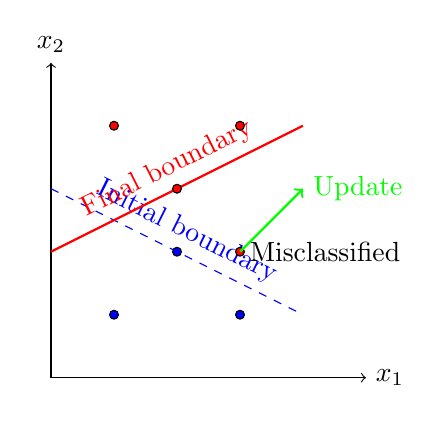
\begin{tikzpicture}[scale=0.8]
    \draw[->] (0,0) -- (5,0) node[right] {$x_1$};
    \draw[->] (0,0) -- (0,5) node[above] {$x_2$};
    
    % Initial boundary
    \draw[dashed, blue] (0,3) -- (4,1) node[midway, above, sloped] {Initial boundary};
    
    % Final boundary
    \draw[thick, red] (0,2) -- (4,4) node[midway, above, sloped] {Final boundary};
    
    % Points
    \draw[fill=red] (1,4) circle (2pt);
    \draw[fill=red] (2,3) circle (2pt);
    \draw[fill=red] (3,4) circle (2pt);
    \draw[fill=blue] (1,1) circle (2pt);
    \draw[fill=blue] (2,2) circle (2pt);
    \draw[fill=blue] (3,1) circle (2pt);
    
    % Misclassified point
    \draw[fill=red] (3,2) circle (2pt) node[right] {Misclassified};
    \draw[->, thick, green] (3,2) -- (4,3) node[right] {Update};
\end{tikzpicture}
\caption{Illustration of a Perceptron update. The misclassified positive point causes the decision boundary to shift.}
\end{figure}

\section{The Perceptron in Action}

\subsection{Example: Linearly Separable Data}
The lecture demonstrated the Perceptron algorithm on a dataset of 85 linearly separable points:
\begin{itemize}
    \item The algorithm was run multiple times with different random orderings of the data
    \item Each run converged to a different linear boundary that perfectly separated the classes
    \item The number of iterations required for convergence varied (e.g., 9, 15, 8, 14 iterations)
\end{itemize}

\subsection{Visualization of Convergence}
\begin{figure}[h]
\centering
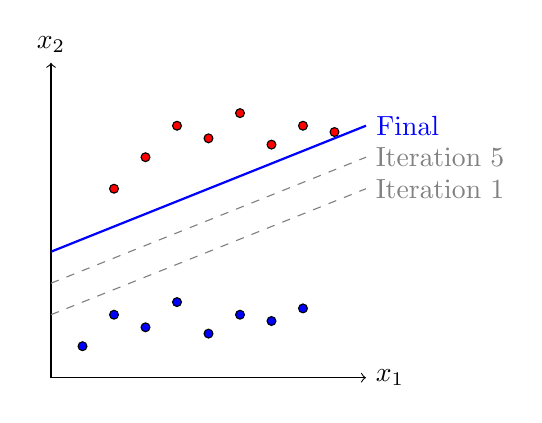
\begin{tikzpicture}[scale=0.8]
    % Coordinate axes
    \draw[->] (0,0) -- (5,0) node[right] {$x_1$};
    \draw[->] (0,0) -- (0,5) node[above] {$x_2$};
    
    % Data points (simplified representation)
    \foreach \x/\y in {0.5/0.5, 1/1, 1.5/0.8, 2/1.2, 2.5/0.7, 3/1, 3.5/0.9, 4/1.1}
        \draw[fill=blue] (\x,\y) circle (2pt);
    
    \foreach \x/\y in {1/3, 1.5/3.5, 2/4, 2.5/3.8, 3/4.2, 3.5/3.7, 4/4, 4.5/3.9}
        \draw[fill=red] (\x,\y) circle (2pt);
    
    % Decision boundaries at different iterations
    \draw[dashed, gray] (0,1) -- (5,3) node[right] {Iteration 1};
    \draw[dashed, gray] (0,1.5) -- (5,3.5) node[right] {Iteration 5};
    \draw[thick, blue] (0,2) -- (5,4) node[right] {Final};
\end{tikzpicture}
\caption{Illustration of Perceptron convergence on linearly separable data. The decision boundary evolves over iterations until it perfectly separates the classes.}
\end{figure}

\section{Convergence Properties}

\subsection{Convergence Theorem}
A fundamental result for the Perceptron algorithm:

\fbox{
\begin{minipage}{\dimexpr\textwidth-2\fboxsep-2\fboxrule\relax}
\textbf{Perceptron Convergence Theorem}

If the training data is linearly separable, then:
\begin{itemize}
    \item The Perceptron algorithm will find a linear classifier with zero training error
    \item It will converge within a finite number of steps
\end{itemize}
\end{minipage}
}

\subsection{Margin and Convergence Rate}
The number of iterations required for convergence depends on the margin:
\begin{itemize}
    \item Margin: A measure of the separation between the two classes
    \item Larger margin → Faster convergence
    \item The upper bound on the number of iterations is proportional to $1/\gamma^2$, where $\gamma$ is the margin
\end{itemize}

\begin{figure}[h]
\centering
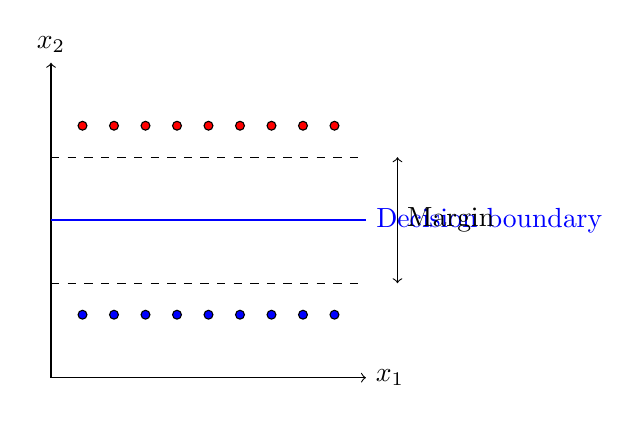
\begin{tikzpicture}[scale=0.8]
    \draw[->] (0,0) -- (5,0) node[right] {$x_1$};
    \draw[->] (0,0) -- (0,5) node[above] {$x_2$};
    
    % Decision boundary
    \draw[thick, blue] (0,2.5) -- (5,2.5) node[right] {Decision boundary};
    
    % Margin
    \draw[dashed] (0,1.5) -- (5,1.5);
    \draw[dashed] (0,3.5) -- (5,3.5);
    \draw[<->] (5.5,1.5) -- (5.5,3.5) node[midway, right] {Margin};
    
    % Points
    \foreach \x in {0.5,1,...,4.5}
        \draw[fill=blue] (\x,1) circle (2pt);
    
    \foreach \x in {0.5,1,...,4.5}
        \draw[fill=red] (\x,4) circle (2pt);
\end{tikzpicture}
\caption{Illustration of margin in a linearly separable dataset. The margin is the distance between the decision boundary and the closest data points.}
\end{figure}

\section{Limitations and Extensions}

\subsection{Non-linearly Separable Data}
The Perceptron algorithm has a significant limitation:
\begin{itemize}
    \item It is only guaranteed to converge if the data is linearly separable
    \item For non-linearly separable data, it may oscillate indefinitely
\end{itemize}

\subsection{Pocket Algorithm}
A simple extension to handle non-linearly separable data:
\begin{itemize}
    \item Run the standard Perceptron algorithm
    \item Keep track of the best weights found so far (those with the lowest training error)
    \item Return these "pocket" weights after a fixed number of iterations
\end{itemize}

\subsection{Kernel Perceptron}
The Perceptron can be extended to handle non-linear decision boundaries using the kernel trick:
\begin{itemize}
    \item Implicitly map the data to a higher-dimensional space where it becomes linearly separable
    \item Apply the Perceptron algorithm in this higher-dimensional space
    \item Common kernels: polynomial, radial basis function (RBF)
\end{itemize}

\begin{figure}[h]
\centering
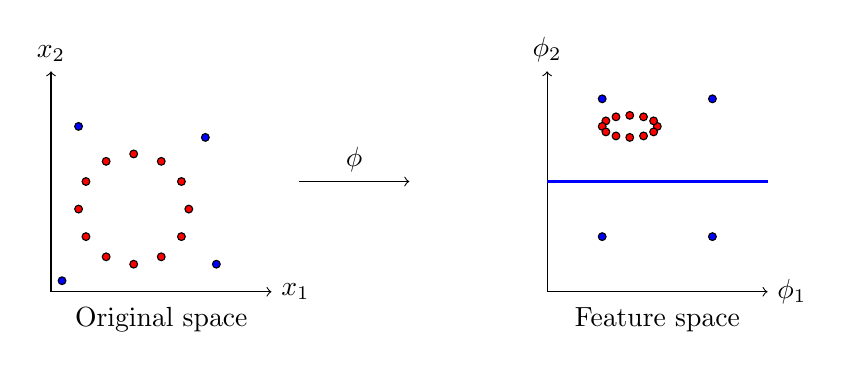
\begin{tikzpicture}[scale=0.7]
    % Original space
    \begin{scope}
        \draw[->] (0,0) -- (4,0) node[right] {$x_1$};
        \draw[->] (0,0) -- (0,4) node[above] {$x_2$};
        
        % Circle of points
        \foreach \angle in {0,30,...,330}
            \draw[fill=red] ({1.5+cos(\angle)},{1.5+sin(\angle)}) circle (2pt);
        
        % Outer points
        \foreach \x/\y in {0.2/0.2, 0.5/3, 3/0.5, 2.8/2.8}
            \draw[fill=blue] (\x,\y) circle (2pt);
        
        \node at (2,-0.5) {Original space};
    \end{scope}
    
    % Arrow
    \draw[->] (4.5,2) -- (6.5,2) node[midway, above] {$\phi$};
    
    % Feature space
    \begin{scope}[xshift=9cm]
        \draw[->] (0,0) -- (4,0) node[right] {$\phi_1$};
        \draw[->] (0,0) -- (0,4) node[above] {$\phi_2$};
        
        % Transformed points
        \foreach \angle in {0,30,...,330}
            \draw[fill=red] ({1.5+0.5*cos(\angle)},{3+0.2*sin(\angle)}) circle (2pt);
        
        \foreach \x/\y in {1/1, 1/3.5, 3/1, 3/3.5}
            \draw[fill=blue] (\x,\y) circle (2pt);
        
        % Linear separator
        \draw[thick, blue] (0,2) -- (4,2);
        
        \node at (2,-0.5) {Feature space};
    \end{scope}
\end{tikzpicture}
\caption{Kernel trick: Mapping non-linearly separable data to a space where it becomes linearly separable}
\end{figure}

\section{Relationship to Neural Networks}

\subsection{The Perceptron as a Neuron}
The Perceptron can be viewed as a single artificial neuron:
\begin{itemize}
    \item Inputs: Feature vector $\mathbf{x}$
    \item Weights: Vector $\mathbf{w}$ and bias $b$
    \item Activation function: Sign function
    \item Output: Binary prediction $\hat{y}$
\end{itemize}

\subsection{Multi-layer Perceptrons}
Modern neural networks extend the Perceptron concept:
\begin{itemize}
    \item Multiple layers of neurons
    \item Differentiable activation functions (e.g., sigmoid, ReLU)
    \item Trained using backpropagation and gradient descent
\end{itemize}

\begin{figure}[h]
\centering
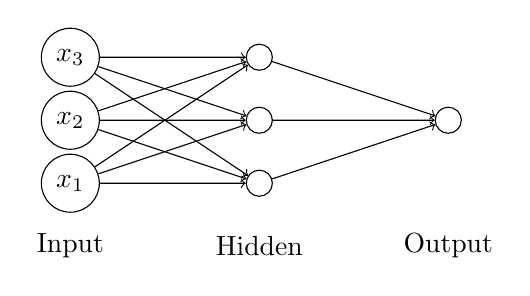
\begin{tikzpicture}[scale=0.8]
    % Input layer
    \foreach \i in {1,2,3} {
        \node[circle, draw] (I\i) at (0,\i) {$x_\i$};
    }
    \node at (0,0) {Input};
    
    % Hidden layer
    \foreach \i in {1,2,3} {
        \node[circle, draw] (H\i) at (3,\i) {};
    }
    \node at (3,0) {Hidden};
    
    % Output layer
    \node[circle, draw] (O1) at (6,2) {};
    \node at (6,0) {Output};
    
    % Connections
    \foreach \i in {1,2,3} {
        \foreach \j in {1,2,3} {
            \draw[->] (I\i) -- (H\j);
        }
    }
    
    \foreach \i in {1,2,3} {
        \draw[->] (H\i) -- (O1);
    }
\end{tikzpicture}
\caption{A multi-layer perceptron with one hidden layer}
\end{figure}

\section{Worked Examples}

\subsection{Example 1: Perceptron Learning on a Simple Dataset}
Consider the following 2D dataset:
\begin{itemize}
    \item Positive examples: $(1,1)$, $(2,2)$
    \item Negative examples: $(1,2)$, $(2,1)$
\end{itemize}

Let's trace through the Perceptron algorithm:

\paragraph{Initialization:} $\mathbf{w} = (0,0)$, $b = 0$

\paragraph{Iteration 1:}
\begin{itemize}
    \item Example $(1,1)$, $y = +1$:
    \begin{align}
        y(\mathbf{w} \cdot \mathbf{x} + b) &= 1 \cdot ((0,0) \cdot (1,1) + 0) = 0 \leq 0
    \end{align}
    Misclassified, so update:
    \begin{align}
        \mathbf{w} &= (0,0) + 1 \cdot (1,1) = (1,1)\\
        b &= 0 + 1 = 1
    \end{align}
    
    \item Example $(2,2)$, $y = +1$:
    \begin{align}
        y(\mathbf{w} \cdot \mathbf{x} + b) &= 1 \cdot ((1,1) \cdot (2,2) + 1) = 5 > 0
    \end{align}
    Correctly classified, no update.
    
    \item Example $(1,2)$, $y = -1$:
    \begin{align}
        y(\mathbf{w} \cdot \mathbf{x} + b) &= -1 \cdot ((1,1) \cdot (1,2) + 1) = -4 < 0
    \end{align}
    Correctly classified, no update.
    
    \item Example $(2,1)$, $y = -1$:
    \begin{align}
        y(\mathbf{w} \cdot \mathbf{x} + b) &= -1 \cdot ((1,1) \cdot (2,1) + 1) = -4 < 0
    \end{align}
    Correctly classified, no update.
\end{itemize}

After one pass through the data, all examples are correctly classified. The final decision boundary is $x_1 + x_2 + 1 = 0$ or $x_2 = -x_1 - 1$.

\subsection{Example 2: Non-convergence on Non-linearly Separable Data}
Consider the XOR problem:
\begin{itemize}
    \item Positive examples: $(0,0)$, $(1,1)$
    \item Negative examples: $(0,1)$, $(1,0)$
\end{itemize}

This dataset is not linearly separable. Let's see what happens with the Perceptron:

\paragraph{Initialization:} $\mathbf{w} = (0,0)$, $b = 0$

\paragraph{Iteration 1:}
\begin{itemize}
    \item Example $(0,0)$, $y = +1$:
    \begin{align}
        y(\mathbf{w} \cdot \mathbf{x} + b) &= 1 \cdot ((0,0) \cdot (0,0) + 0) = 0 \leq 0
    \end{align}
    Misclassified, so update:
    \begin{align}
        \mathbf{w} &= (0,0) + 1 \cdot (0,0) = (0,0)\\
        b &= 0 + 1 = 1
    \end{align}
    
    \item Example $(1,1)$, $y = +1$:
    \begin{align}
        y(\mathbf{w} \cdot \mathbf{x} + b) &= 1 \cdot ((0,0) \cdot (1,1) + 1) = 1 > 0
    \end{align}
    Correctly classified, no update.
    
    \item Example $(0,1)$, $y = -1$:
    \begin{align}
        y(\mathbf{w} \cdot \mathbf{x} + b) &= -1 \cdot ((0,0) \cdot (0,1) + 1) = -1 < 0
    \end{align}
    Correctly classified, no update.
    
    \item Example $(1,0)$, $y = -1$:
    \begin{align}
        y(\mathbf{w} \cdot \mathbf{x} + b) &= -1 \cdot ((0,0) \cdot (1,0) + 1) = -1 < 0
    \end{align}
    Correctly classified, no update.
\end{itemize}

At this point, $\mathbf{w} = (0,0)$ and $b = 1$, which classifies everything as positive. This is clearly not correct for the negative examples. If we continue iterating, the algorithm will keep updating without converging to a solution that correctly classifies all examples.

\section{Practical Considerations}

\subsection{Initialization}
While the standard Perceptron initializes $\mathbf{w} = \mathbf{0}$ and $b = 0$, different initializations can lead to different solutions and convergence rates.

\subsection{Data Ordering}
The order in which training examples are processed can significantly impact:
\begin{itemize}
    \item The number of iterations required for convergence
    \item The specific decision boundary found
\end{itemize}
Randomizing the order of examples between epochs is a common practice.

\subsection{Learning Rate}
While the standard Perceptron uses a learning rate of 1, a smaller learning rate can sometimes lead to more stable convergence, especially in noisy settings.

\subsection{Feature Scaling}
As with most linear models, the Perceptron benefits from feature scaling:
\begin{itemize}
    \item Standardization: $x' = \frac{x - \mu}{\sigma}$
    \item Min-max scaling: $x' = \frac{x - \min(x)}{\max(x) - \min(x)}$
\end{itemize}

\section{Summary and Key Takeaways}

\subsection{Core Concepts}
\begin{itemize}
    \item The Perceptron is an algorithm for learning linear classifiers
    \item It updates the model parameters only when a misclassification occurs
    \item The update rule is simple: add the feature vector (scaled by the label) to the weight vector
    \item For linearly separable data, the Perceptron is guaranteed to converge in a finite number of steps
\end{itemize}

\subsection{Strengths}
\begin{itemize}
    \item Simple and intuitive algorithm
    \item Guaranteed convergence for linearly separable data
    \item Online learning capability (can process one example at a time)
    \item Historically significant as a foundation for neural networks
\end{itemize}

\subsection{Limitations}
\begin{itemize}
    \item Only works for linearly separable data
    \item No convergence guarantee for non-linearly separable data
    \item The solution depends on the order of training examples
    \item Does not provide probability estimates
\end{itemize}

\subsection{Extensions and Related Concepts}
\begin{itemize}
    \item Pocket Algorithm for non-linearly separable data
    \item Kernel Perceptron for non-linear decision boundaries
    \item Multi-layer Perceptrons and neural networks
    \item Support Vector Machines for maximum-margin linear classification
\end{itemize}

\end{document}